\chapter{Robotic System and Experimental Setup}\label{ch:rob_setup}

This chapter describes the physical experimental platform used for the data acquisition in this thesis. The setup consists of an industrial robot manipulator, a parallel gripper with interchangeable finger configurations, multiple insertion rods, a custom taskboard containing the matching geometries, and a loadcell-based success detection mechanism mounted below the taskboard. Together, these components form the basis for the automated execution and evaluation of insertion attempts. While this chapter focuses on the hardware configuration and the functional role of each component, the data acquisition procedure and the dataset generation pipeline are described in the next Chapter~\ref{ch:dataset}.

\section{Robotic System Overview}\label{sec:rob_setup-overview}

The experimental setup is built around a UR5e robotic manipulator equipped with a Robotiq Hand-E gripper to its endeffector. The robot repeatedly picks-up a rod from the holder, which is builtin into the taskboard stand, and inserts it into the corresponding hole, while recording all relevant data. A photo of the full setup is shown in Figure~\ref{fig:setup_overview}, and a schematic overview of the main components is provided in Figure~\ref{fig:setup_schematic}.

\begin{figure}[htbp]
    \centering
    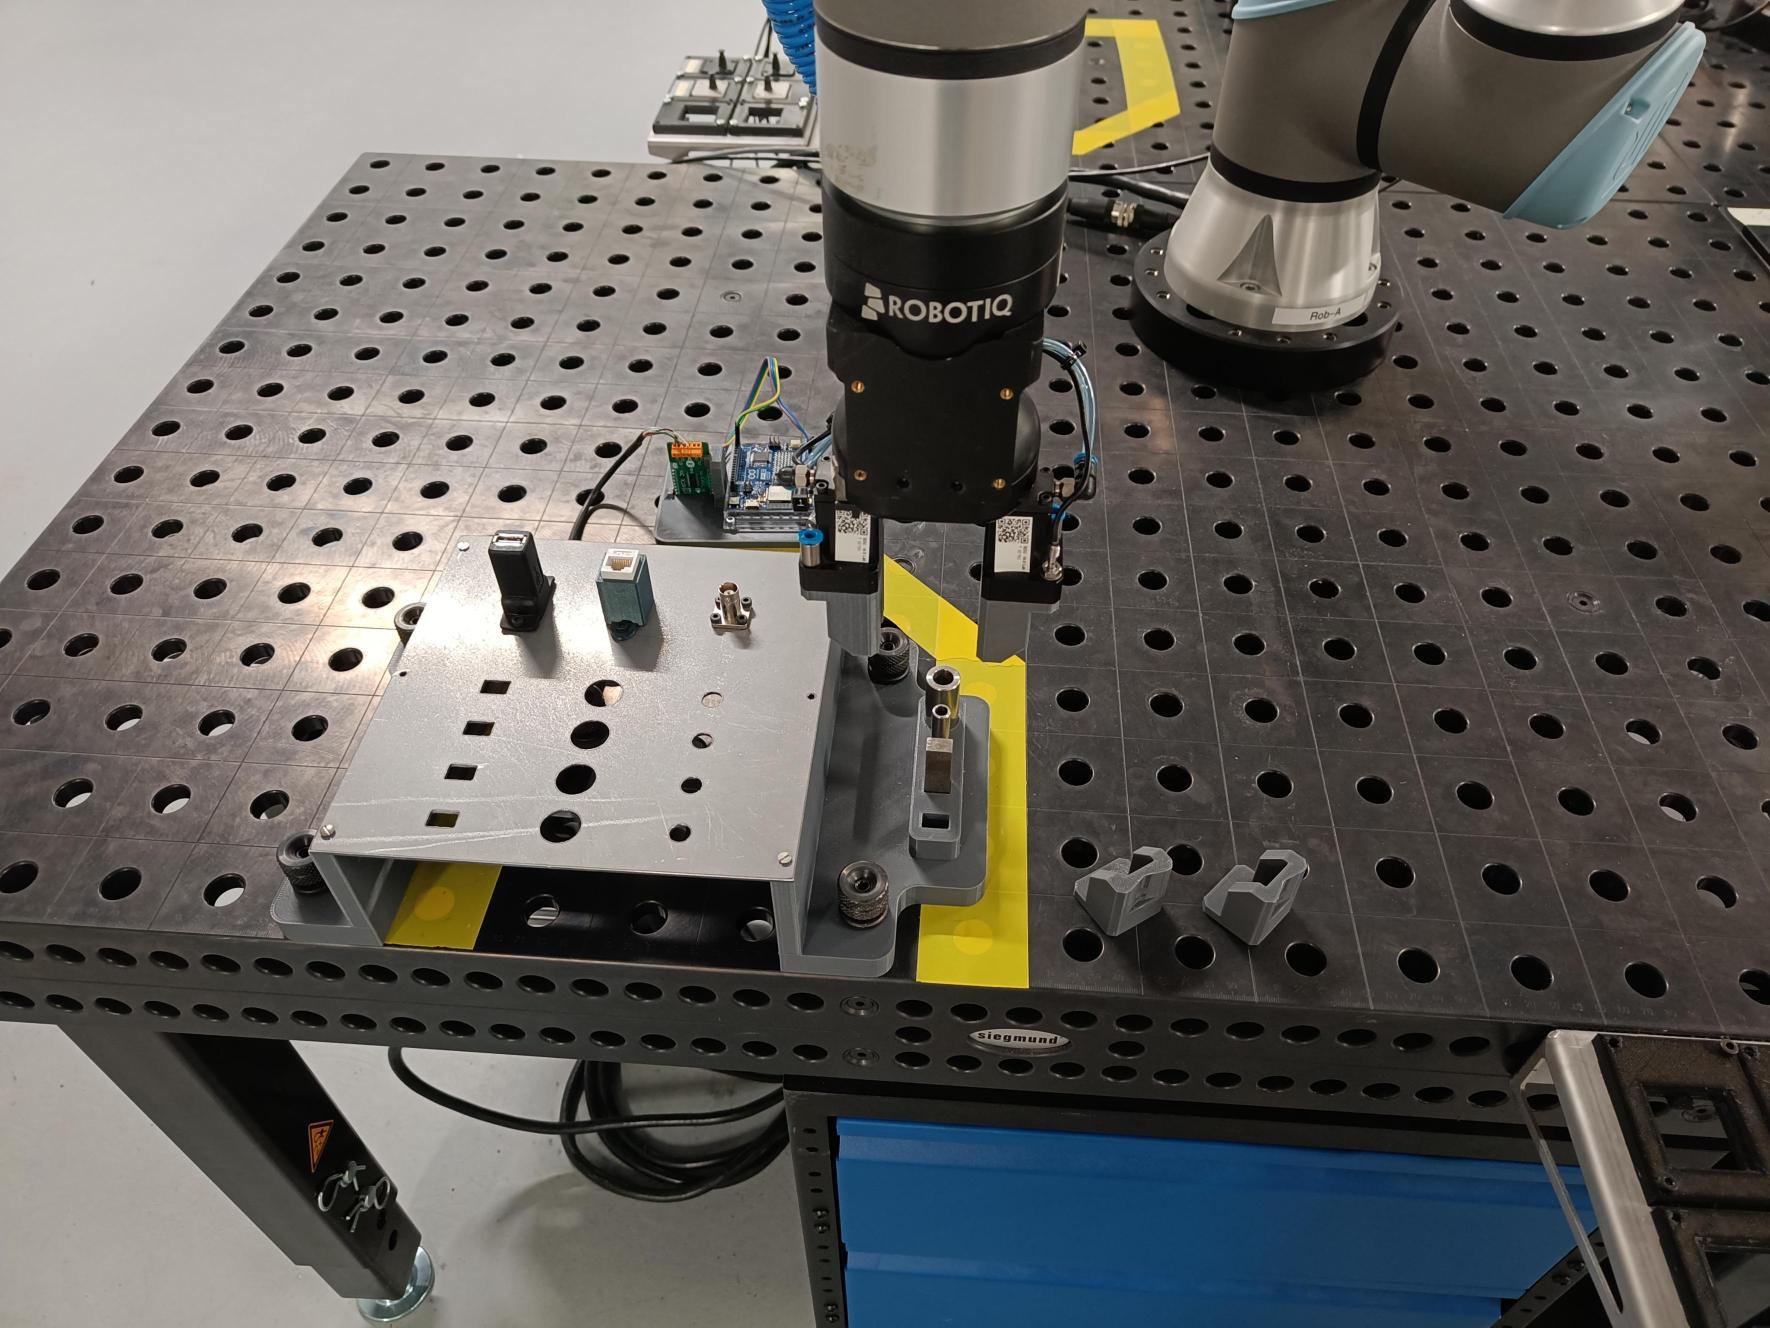
\includegraphics[width=0.9\textwidth]{chapters/3-robotic_system_and_experimental_setup/rob_setup_3.jpeg}
    \caption{Overview of the experimental setup showing the UR5e robot, Robotiq Hand-E gripper, and taskboard with the loadcell underneath.}
    \label{fig:setup_overview}
\end{figure}

\begin{figure}[htbp]
    \centering
    % \includegraphics[width=0.9\textwidth]{[PATH_TO_SETUP_SCHEMATIC]}
    \caption{Schematic representation of the main hardware components and their arrangement.}
    \label{fig:setup_schematic}
\end{figure}

For the experimenst the UR5e robot was selected due to its ease of use, broad availability combined with sufficient accuracy to achieve repeatable cartesian motion to perform the insertions. Since the robot itself is not the subject of investigation in this work, only its functional role within the setup is considered here. Similarly, the Robotiq Hand-E gripper is used to reliably grasp and release the insertion rods and furthermore allow different shapes of rods to be grasped due to interchangeable and fully customizable fingers. Different finger configurations were designed to ensure safe grasping of the respective rod types while also allowing little play to generate diverse training data. The specific rod and finger geometries are described in Section~\ref{sec:rods-fingers}.

The robot interacts with a custom taskboard mounted next to it. The taskboard contains the respective insertion holes with a movable loadcell underneath to detect successful insertions, which enables automated success detection during data acquisition. The taskboard design is described in Section~\ref{sec:taskboard}, while the loadcell-based success detection system is presented in Section~\ref{sec:loadcell}.

\section{Insertion Rods and Gripper Fingers}\label{sec:rods-fingers}

The insertion tasks consists of a set of custom insertion rods with different cross-sectional geometries. In total 3 rod types are used: 
\begin{enumerate}
    \item Small Rod with $8.8$ mm diameter
    \item Big Rod with $15.8$ mm diameter
    \item Rectangular Rod with side length $12\times8$ mm
\end{enumerate}
These shapes were picked to represent common insertion conditions while still providing comparable results. Figure~\ref{fig:rods_overview} shows the 3 rods used in this work. All rods are $50$ mm long and machined out of steel.

\begin{figure}[htbp]
    \centering
    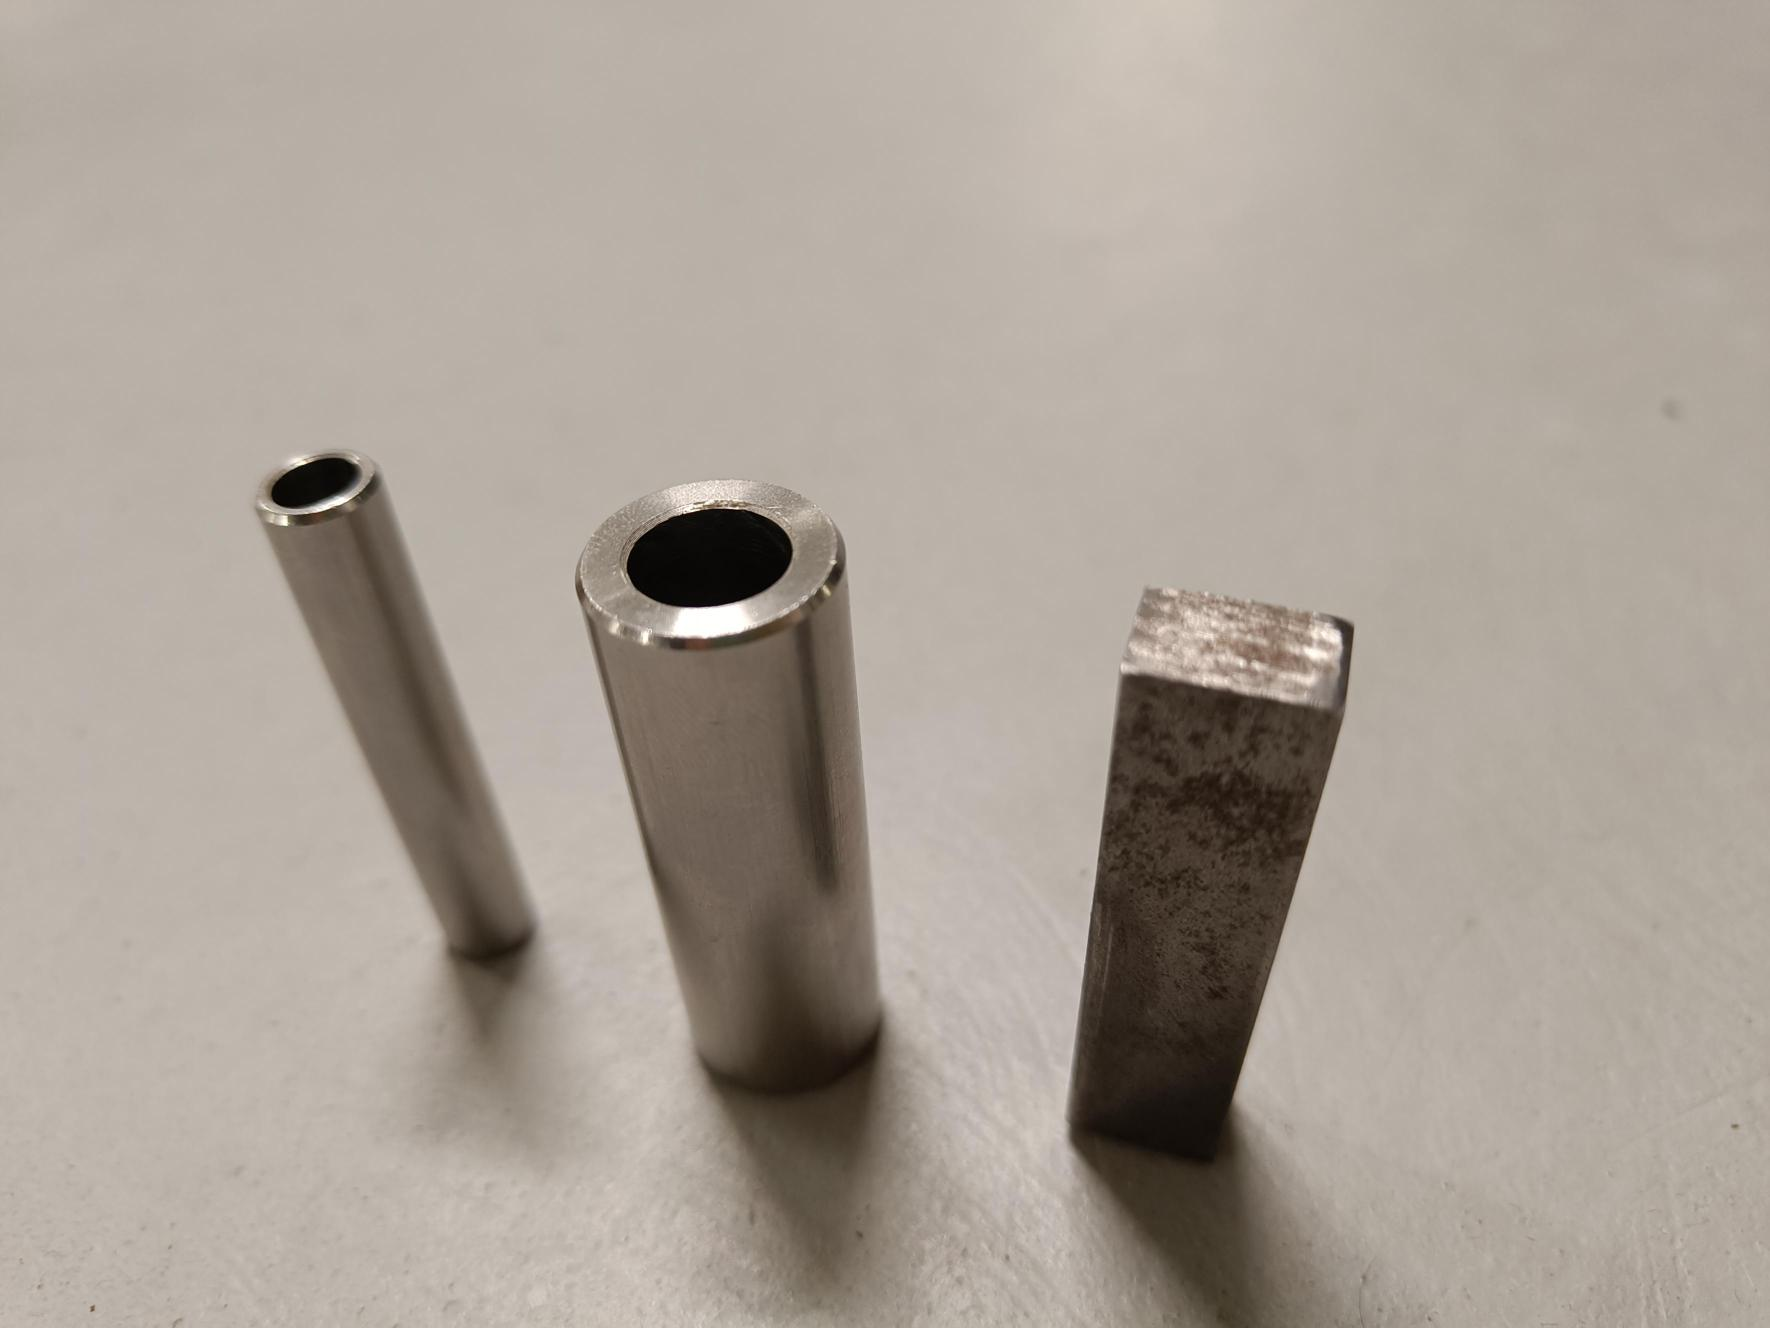
\includegraphics[width=0.9\textwidth]{chapters/3-robotic_system_and_experimental_setup/rods_overview.jpeg}
    \caption{Insertion rod geometries used for the experiments. Left to right: Small Rod, Big Rod, Rectangular Rod.}
    \label{fig:rods_overview}
\end{figure}

Since the different rods could not be grasped equally well using a single finger geometry, three dedicated gripper finger configurations were used. The fingers were designed to provide secure and repeatable grasps for the respective rod types while minimizing undesired motion of the rod relative to the gripper during insertion.

A representative overview of the finger designs is shown in Figure~\ref{fig:finger_designs}. Depending on the available visual material, either CAD renderings, technical drawings, or photographs of the mounted fingers can be used here. For the purposes of this thesis, the important aspect is not the full manufacturing detail of the fingers, but their functional relation to the rod geometries.

\begin{figure}[htbp]
    \centering
    % \includegraphics[width=0.9\textwidth]{[PATH_TO_FINGER_FIGURE]}
    \caption{Interchangeable gripper finger configurations used for grasping the different insertion rods.}
    \label{fig:finger_designs}
\end{figure}

If relevant, the grasping concept can additionally be summarized in Table~\ref{tab:finger_assignment}.

\begin{table}[htbp]
    \centering
    \caption{Assignment of rod geometries to gripper finger configurations.}
    \label{tab:finger_assignment}
    \begin{tabular}{lll}
        \hline
        Rod ID & Finger configuration & Functional purpose \\
        \hline
        [ROD\_1] & [FINGER\_A] & [e.g.\ centered pinch grasp] \\
        jo & [FINGER\_B] & [e.g.\ improved support for rectangular profile] \\
        jo & [FINGER\_C] & [e.g.\ increased contact stability] \\
        \hline
    \end{tabular}
\end{table}

\section{Taskboard}\label{sec:taskboard}

The mating features for the insertion experiments are integrated into a custom taskboard. The taskboard serves as the central interaction object of the experimental setup and defines the physical insertion conditions for all recorded trials. A CAD rendering of the taskboard is shown in Figure~\ref{fig:taskboard_cad}, followed by a photograph of the manufactured assembly in Figure~\ref{fig:taskboard_real}.

\begin{figure}[htbp]
    \centering
    % \includegraphics[width=0.9\textwidth]{[PATH_TO_TASKBOARD_CAD]}
    \caption{CAD model of the taskboard used for the insertion experiments.}
    \label{fig:taskboard_cad}
\end{figure}

\begin{figure}[htbp]
    \centering
    % \includegraphics[width=0.9\textwidth]{[PATH_TO_TASKBOARD_PHOTO]}
    \caption{Manufactured taskboard integrated into the experimental setup.}
    \label{fig:taskboard_real}
\end{figure}

The taskboard contains insertion features corresponding to the rod geometries described in Section~\ref{sec:rods-fingers}. For each geometry, multiple tolerance variants were implemented in order to generate insertion tasks with different levels of difficulty. This allows the dataset to cover a broader range of contact interactions and insertion outcomes while preserving a controlled and comparable experimental environment.

The selected tolerance levels were chosen to create distinguishable insertion conditions without changing the task principle itself. In this way, the influence of geometric fit on the recorded force and torque signatures can be investigated systematically. The exact tolerance values used for each feature are summarized in Table~\ref{tab:taskboard_tolerances}.

\begin{table}[htbp]
    \centering
    \caption{Insertion features and tolerance levels implemented in the taskboard.}
    \label{tab:taskboard_tolerances}
    \begin{tabular}{llll}
        \hline
        Feature ID & Rod geometry & Nominal dimension / fit & Tolerance \\
        \hline
        [FEATURE\_1] & [GEOMETRY] & [VALUE] & [e.g.\ $\pm 0.1$ mm] \\
        jo & [GEOMETRY] & [VALUE] & [e.g.\ $\pm 0.2$ mm] \\
        jo & [GEOMETRY] & [VALUE] & [e.g.\ $\pm 0.3$ mm] \\
        \hline
    \end{tabular}
\end{table}

In addition to the rod-based insertion features, the taskboard also includes mounting provisions for snap-fit experiments. These features were part of the original taskboard design because snap-fit assembly was initially considered as a second task family. However, snap-fit trials were not included in the final dataset used in this thesis. The main reason for this decision was to keep the scope of data acquisition manageable while maintaining sufficient data volume per task variant. In addition, reliable automatic label assignment is more straightforward for the rod insertion tasks, since successful completion can be detected mechanically by the loadcell system described in Section~\ref{sec:loadcell}. For snap-fit tasks, defining an equally robust external success criterion would have required additional sensing or validation steps. Therefore, the final experiments in this thesis focus exclusively on rod insertion tasks.

\section{Loadcell-Based Success Detection}\label{sec:loadcell}

To enable automated label assignment during data acquisition, the setup includes a loadcell mounted underneath the taskboard. The purpose of this subsystem is to detect whether an insertion rod has passed through the corresponding taskboard feature far enough to mechanically contact the loadcell target beneath the board. In the experimental logic of this work, such a contact event is interpreted as a successful insertion.

A schematic side view of the loadcell integration is shown in Figure~\ref{fig:loadcell_concept}. If available, this figure should illustrate the relation between the taskboard, the insertion rod, and the loadcell position below the board.

\begin{figure}[htbp]
    \centering
    % \includegraphics[width=0.8\textwidth]{[PATH_TO_LOADCELL_SCHEMATIC]}
    \caption{Principle of loadcell-based success detection below the taskboard.}
    \label{fig:loadcell_concept}
\end{figure}

Mechanically, the loadcell is mounted below the taskboard using a dedicated support structure attached to the main experimental frame or table. [ADD ONE SENTENCE HERE DESCRIBING THE MOUNTING PRINCIPLE, e.g.\ whether a 3D-printed bracket was used and whether vertical alignment was adjustable.] The exact geometry of the mounting hardware is not critical to the understanding of the experiment, provided that the position of the sensing element relative to the taskboard is reproducible and mechanically stable.

The loadcell used in this work is a [LOADCELL PART NUMBER / TYPE / NOMINAL RANGE] and is connected to a dedicated loadcell analog-to-digital converter, namely [ADC PART NUMBER]. The converter is interfaced with an Arduino Uno R4 WiFi, which samples the sensor signal at approximately [SAMPLING RATE]~Hz. The measured loadcell value is transmitted wirelessly to the recording computer, where it is monitored during data acquisition.

At the level relevant for this chapter, the signal processing principle is intentionally simple: when the transmitted loadcell value exceeds a predefined threshold of [THRESHOLD VALUE AND UNIT], the corresponding trial is marked as successful. This approach provides a direct and hardware-based success signal that can be used for automated labelling. The detailed recording implementation, synchronization with the robot data stream, and the final labelling pipeline are described in Chapter~\ref{[LABEL_OF_CH4]}.

The loadcell subsystem is included specifically to avoid purely manual success annotation and to provide a reproducible criterion for successful insertion. Since the success label plays a central role in the dataset generation, the sensor placement and thresholding principle are experimentally important even though the underlying microcontroller and communication implementation are not themselves the focus of this thesis.